\documentclass{article}

% NeurIPS 2026 submission (Main Track, double-blind, with line numbers).
\usepackage{neurips_2026}

\usepackage[utf8]{inputenc}
\usepackage[T1]{fontenc}
\usepackage{hyperref}
\usepackage{url}
\usepackage{booktabs}
\usepackage{amsfonts}
\usepackage{amsmath}
\usepackage{amssymb}
\usepackage{amsthm}
\usepackage{nicefrac}
\usepackage{microtype}
\usepackage{xcolor}
\usepackage{graphicx}
\usepackage{caption}
\usepackage{subcaption}
\usepackage{cleveref}

\graphicspath{{../figures/out/}{../figures/out/appendix/}}

\newtheorem{theorem}{Theorem}
\newtheorem*{theorem*}{Theorem}
\newtheorem{proposition}{Proposition}
\newtheorem{lemma}{Lemma}
\newtheorem{corollary}{Corollary}
\newtheorem{definition}{Definition}

\title{The Bellman Residual Is Not the Improvement Signal}

% Anonymous author block is rendered automatically by the neurips_2026 style
% file in submission mode. Do not deanonymize here.
\author{%
  Anonymous Author(s) \\
  Affiliation \\
  Address \\
  \texttt{email}
}

\begin{document}
\maketitle

\begin{abstract}
Actor--critic methods typically assess critic quality using the Bellman residual $\epsilon_u$ computed on rollout states. We argue that this quantity is misaligned with policy improvement: it is measured on the wrong distribution and at the wrong scale. We establish an exact identity, $J(\pi_{k+1}) - J(\pi_k) = A_k - \hat\Delta_k$, where $\hat\Delta_k := J(\pi_k) - \mathbb{E}_{s \sim \nu}[V_{k+1}(s)]$ measures the start-state bias of the post-update critic. The Bellman residual does not appear in the improvement decomposition. We further prove a structural limitation: any fixed absolute tolerance on $\epsilon_u$ becomes uninformative as $\pi_k$ converges and $A_k \to 0$, rendering it unable to certify progress regardless of magnitude.

Empirically, across $\sim$90{,}000 updates spanning four configurations (PPO, PPO-MSE, SAC, TRPO) on up to eight environments (263 seeds total), we find that $-\widehat\epsilon_u$ is not predictive of harmful updates (pooled median AUROC 0.47), while $-\widehat{\hat\Delta}_k$ achieves stronger predictive performance (0.68) and dominates $-\widehat\epsilon_u$ on 256 of 262 paired seeds ($p < 10^{-43}$). We also observe that the surrogate advantage $A_k$ optimized by PPO can become anti-predictive in complex environments (pooled median AUROC 0.39), consistent with overfitting effects that inflate $A_k$ when start-state bias is large. Finally, an additive $\nu$-weighted critic-loss intervention (PPO-NU) fails to make $\hat\Delta_k$ prospective, suggesting that the mismatch is not closeable by simple reweighting of a rollout-fit loss. These results suggest that actor--critic monitoring and critic-loss design should move beyond rollout-distribution residuals toward start-state-aware quantities.
\end{abstract}

\section{Introduction}
\label{sec:intro}

Actor--critic algorithms in deep reinforcement learning (RL)---PPO \citep{schulman2017proximal}, SAC \citep{haarnoja2018soft}, TRPO \citep{schulman2015trust}---update a policy iteratively against a learned value function. The critic is fit, monitored, and \emph{judged} by its mean squared TD error on the rollout distribution $d^{\pi_k}$: this is the loss every implementation we surveyed minimizes \citep{huang202237,andrychowicz2021what}, and the scalar practitioners watch to decide whether the critic is ``good enough'' to support policy improvement.

\paragraph{The structural problem.}
Policy improvement, however, is not governed by critic error on $d^{\pi_k}$. The expected return $J(\pi) = \mathbb{E}_{s_0 \sim \nu}[V^\pi(s_0)]$ involves the critic only through its accuracy at the start-state distribution $\nu$. The two distributions are not the same: $d^{\pi_k}$ is the discounted state-visitation distribution from $\nu$, and the difference is non-trivial even on-policy. Actor--critic methods therefore optimize and certify a critic on the wrong distribution.

The consequence is not merely that $\epsilon_u$ is a noisy proxy, but that it is often at the wrong scale. As the policy converges and $A_k \to 0$, any fixed absolute $\epsilon_u$ tolerance eventually encodes a return scale larger than the remaining improvement signal, precluding prospective certification. The work below makes this consequence exact, then confirms it empirically at scale.

\paragraph{Distinction from prior treatments.}
While classical on-policy improvement bounds treat the $d^\pi$/$\nu$ mismatch as an approximation gap closed by importance-ratio reweighting or trust-region constraints, we show it is a structural fact. The identity below eliminates $\epsilon_u$ entirely at the population level, exposing the residual scaffolding of prior bounds as unnecessary, and fixing a new target for future critic-loss design.

\paragraph{The identity that eliminates the Bellman residual.}
The mismatch admits an exact algebraic resolution. For \emph{any} value function $V_{k+1}$,
\begin{equation}
\label{eq:identity-intro}
J(\pi_{k+1}) - J(\pi_k) \;=\; A_k \;-\; \hat\Delta_k,\qquad
\hat\Delta_k := J(\pi_k) - \mathbb{E}_{s \sim \nu}[V_{k+1}(s)].
\end{equation}
This is not a bound and not an explanation. It is the ground-truth decomposition of policy improvement, and it reveals why the standard monitor $\epsilon_u$ is fundamentally misaligned with the objective: the Bellman residual does not appear in the improvement decomposition at all. While classical bounds introduce $\epsilon_u$ as scaffolding, the exact algebraic resolution shows the start-state bias $\hat\Delta_k$ is the operative quantity. Furthermore, as we show in \Cref{sec:theory}, $\epsilon_u$ is also at the wrong \emph{scale}: the relevant tolerance is $\epsilon_u / A_k$, so any fixed absolute tolerance eventually fails to certify even genuine improvement as $A_k \to 0$.

\paragraph{Empirical confirmation across $\sim$90{,}000 updates.}
The structural prediction is unambiguous: $\epsilon_u$ should not track policy improvement, and $\hat\Delta_k$ should. We audit $263$ seeds across PPO, the PPO-MSE ablation, SAC, and TRPO on up to eight environments. Because $\epsilon_u$ measures critic error correctly, but on the wrong distribution, it is \emph{anti-predictive} of policy harm (pooled median AUROC $0.47$, below chance --- informative but with the wrong sign). Because $\hat\Delta_k$ reflects the actual covariate shift, it pools to $0.68$ and dominates $\epsilon_u$ on $\mathbf{256\,\text{of}\,262}$ paired seeds (paired Wilcoxon $p < 10^{-43}$). The dominance is uniform across all four configurations, robust across a $170$-run hyperparameter factorial, and survives on fully independent held-out rollouts (AUROC $0.61$). This mismatch leads to an ``$A_k$ paradox'' where the surrogate advantage $A_k$ optimized by PPO can become anti-predictive in complex environments (pooled median AUROC 0.39).

\paragraph{The mismatch is not closeable by reweighting.}
We further show that adding an explicit start-state penalty to the critic loss fails to make $\hat\Delta_k$ prospective, suggesting this mismatch is not a deficiency of MSE, but an intrinsic limitation of the actor--critic optimization order (see \Cref{sec:intervention}).

\section{Related work}
\label{sec:related}

\paragraph{Policy-improvement bounds and the on-policy gap.}
Classical on-policy improvement bounds --- CPI \citep{kakade2002approximately}, RPI \citep{pirotta2013relative}, TRPO \citep{schulman2015trust}, and CPO \citep{achiam2017constrained} --- confront the same $d^\pi$/$\nu$ mismatch we identify. Each handles it by a change-of-measure argument: importance-ratio reweighting of the surrogate advantage (CPI) or a trust-region/$D_{\mathrm{KL}}$ constraint that keeps consecutive rollout distributions close (TRPO, CPO). The mismatch survives in the form of a residual scaffolding term proportional to $\epsilon_u$ scaled by an unknown density ratio. The identity in \Cref{prop:identity} shows this scaffolding is unnecessary at the population level: the gap admits an exact algebraic resolution that eliminates $\epsilon_u$ and isolates the start-state bias as the operative quantity. The complementary off-policy distribution-shift and offline RL literature \citep{islam2019off, nachum2019dualdice, voloshin2021empirical, prudencio2023survey} addresses a related but distinct mismatch (behavior vs.\ target policy) often via stationary distribution corrections; however, the gap we identify persists even strictly on-policy. 

\paragraph{Critic failure in deep RL.}
Empirically, \citet{ilyas2020closer} established that deep RL critics often fail to fit the true value function even on-policy, observing that the network often solves the supervised task (minimizing TD error) without solving the estimation problem (predicting returns). \citet{andrychowicz2021what} further confirmed that value-loss is poorly correlated with agent performance across a large-scale PPO study. Our identity (\Cref{prop:identity}) provides the structural explanation for these empirical findings: because value-loss is minimized over the wrong distribution ($d^\pi$), it is dimensionally and structurally decoupled from the start-state error ($\hat\Delta_k$) that actually governs the improvement signal.


\section{The central lens: an exact identity at the start-state distribution}
\label{sec:setup}

We consider an infinite-horizon discounted MDP $(\mathcal{S}, \mathcal{A}, P, R, \gamma, \nu)$ with state space $\mathcal{S}$, action space $\mathcal{A}$, transition kernel $P : \mathcal{S} \times \mathcal{A} \to \Delta(\mathcal{S})$, reward $R$, discount $\gamma \in [0, 1)$, and initial-state distribution $\nu \in \Delta(\mathcal{S})$. For a policy $\pi$, write $V^\pi$ for its value function, $J(\pi) = \mathbb{E}_{s_0 \sim \nu}[V^\pi(s_0)]$ for its expected return, $T^\pi$ for the Bellman operator, and $d^\pi$ for the discounted state-visitation distribution from $\nu$:
\begin{equation*}
(T^\pi V)(s) = \mathbb{E}_{a \sim \pi}\!\big[R(s,a) + \gamma \mathbb{E}_{s'}[V(s')]\big], \qquad
(d^\pi)^\top = (1-\gamma) \,\nu^\top (I - \gamma P^\pi)^{-1}.
\end{equation*}
Consider an iterative algorithm that, at iteration $k$, holds $\pi_k$ and a critic estimate $V_k$, and produces $(\pi_{k+1}, V_{k+1})$. The estimate $V_{k+1}$ need not coincide with $V^{\pi_{k+1}}$.

\begin{proposition}[Improvement identity at the initial-state distribution]
\label{prop:identity}
For any policies $\pi_k, \pi_{k+1}$ and any value function $V_{k+1} : \mathcal{S} \to \mathbb{R}$,
\begin{equation}
\label{eq:identity}
J(\pi_{k+1}) - J(\pi_k) \;=\; A_k \;-\; \hat\Delta_k,
\end{equation}
where
\begin{equation}
\label{eq:Ak-dhat}
A_k := \tfrac{1}{1-\gamma}\, \mathbb{E}_{s \sim d^{\pi_{k+1}}}\!\left[(T^{\pi_{k+1}} V_{k+1})(s) - V_{k+1}(s)\right]
\;\text{and}\;
\hat\Delta_k := J(\pi_k) - \mathbb{E}_{s \sim \nu}[V_{k+1}(s)].
\end{equation}
\end{proposition}

\begin{proof}
The Bellman residual at $\pi_{k+1}$ on $V_{k+1}$ is $T^{\pi_{k+1}} V_{k+1} - V_{k+1} = r^{\pi_{k+1}} + \gamma P^{\pi_{k+1}} V_{k+1} - V_{k+1}$. Substituting $(d^{\pi_{k+1}})^\top = (1-\gamma) \nu^\top (I - \gamma P^{\pi_{k+1}})^{-1}$ gives
\begin{equation*}
A_k
= \nu^\top (I - \gamma P^{\pi_{k+1}})^{-1} \big(r^{\pi_{k+1}} - (I - \gamma P^{\pi_{k+1}}) V_{k+1}\big)
= J(\pi_{k+1}) - \mathbb{E}_\nu V_{k+1}.
\end{equation*}
Subtracting $\hat\Delta_k = J(\pi_k) - \mathbb{E}_\nu V_{k+1}$ gives $A_k - \hat\Delta_k = J(\pi_{k+1}) - J(\pi_k)$.
\end{proof}


The identity is algebraically equivalent to the Performance Difference Lemma \citep{kakade2002approximately} with $V_{k+1}$ substituted for $V^{\pi_k}$ and rearranged to make $\hat\Delta_k$ explicit. The insight is not the rearrangement but its consequence: $\epsilon_u$ is eliminated from the improvement signal at the population level. Why has $\epsilon_u$ persisted as the standard diagnostic despite PDL being textbook? We find that $\epsilon_u$ and $\hat\Delta_k$ are sufficiently correlated during high-entropy early training (median Spearman $\rho=0.52$ on Humanoid-v5) that the monitor failure is masked while improvement is large. The mismatch manifests only near convergence --- exactly when monitoring matters most.

The identity is exact for any $V_{k+1}$ --- we verify it holds to machine precision in tabular RandomMDPs (\Cref{app:tabular}, median residual $5{\times}10^{-16}$). It is not a bound, not a forecasting claim, and contains no Bellman-residual term. The classical CPI/TRPO bound \citep{kakade2002approximately,schulman2015trust} introduces $\epsilon_u$ only as scaffolding for a change-of-measure step from $d^{\pi_k}$ to $\nu$; once the conversion is done exactly, $\epsilon_u$ vanishes and the start-state bias $\hat\Delta_k$ is what remains. The price is that $\hat\Delta_k$ depends on the post-update critic and is retrospective; the gain is that nothing about critic accuracy on $d^{\pi_k}$ enters at all. Throughout the rest of the paper we treat $\hat\Delta_k$ --- not the full identity remainder --- as the diagnostic of interest, since the empirical work below shows the predictive signal lives almost entirely in this term.

\paragraph{Practical estimators.}
In a deep RL implementation, the population quantities of \Cref{eq:Ak-dhat} are not directly observable. Note that while the exact population identity (\Cref{eq:identity}) requires the post-update critic $V_{k+1}$, standard deep RL implementations compute the surrogate $\widehat{A}_k$ via GAE using the pre-update critic $V_k$. We evaluate the standard estimator to reflect the actual optimization signal utilized in practice. The estimators we use are:
\begin{align}
\label{eq:Ak-est}
\widehat{A}_k
  &\;:=\; \mathbb{E}_{(s,a) \sim B_k}\!\left[\,
      \tfrac{\pi_{k+1}(a \mid s)}{\pi_k(a \mid s)}\,\hat A^{\,\mathrm{GAE}}_{V_k}(s, a)
    \right],\\[0.2em]
\label{eq:dhat-est}
\widehat{\hat\Delta}_k
  &\;:=\; \widehat{J}(\pi_k) \;-\; \tfrac{1}{N_{\text{eps}}}\sum_{i=1}^{N_{\text{eps}}} V_{k+1}(s_0^{(i)}), \\[0.2em]
\label{eq:delta-hat-res}
\widehat{\hat\Delta}^{\,\mathrm{res}}_k
  &\;:=\; \frac{1}{1-\gamma}\,\mathbb{E}_{(s,a,s') \sim B_k}\!\left[r(s,a) + \gamma V_{k+1}(s') - V_{k+1}(s)\right].
\end{align}
Here $B_k$ is the on-policy rollout batch under $\pi_k$, $\hat A^{\,\mathrm{GAE}}$ is the GAE \citep{schulman2015high} advantage at the pre-update critic $V_k$, $\widehat{J}(\pi_k)$ is the mean episode return on the rollout, and $N_{\text{eps}}$ is the number of episodes sampled in the rollout, with $s_0^{(i)}$ being the start state of the $i$-th episode. We adopt the start-state form \Cref{eq:dhat-est} for $\widehat{\hat\Delta}_k$ throughout; the alternative residual-based estimator \Cref{eq:delta-hat-res} has lower per-update variance but agrees only in expectation (\Cref{app:agreement}). The estimator $\widehat{\hat\Delta}_k$ is biased relative to the population $\hat\Delta_k$ because $\widehat{J}(\pi_k)$ has finite-sample variance, and the rollout-conditional start-state mean diverges from the true unconditional expectation $\mathbb{E}_\nu$.


\section{Audit setup}
\label{sec:audit}

We audit four actor--critic configurations spanning three algorithm families.

\paragraph{Algorithms and environments.}
PPO \citep{schulman2017proximal} on the canonical 8-environment suite at $200$k--$500$k timesteps each: discrete-action LunarLander-v3, CartPole-v1, Acrobot-v1, and MuJoCo continuous control on MuJoCo \citep{todorov2012mujoco} Hopper-v5, HalfCheetah-v5, Walker2d-v5, Ant-v5, Humanoid-v5; 20 seeds per environment ($160$ runs). PPO-MSE: an ablation that replaces PPO's clipped value loss with a pure mean-squared TD error, on the same 8 envs $\times$ 5 seeds. SAC \citep{haarnoja2018soft} on five MuJoCo environments (Hopper-v5, HalfCheetah-v5, Walker2d-v5, Ant-v5, Humanoid-v5), $6$--$10$ seeds each ($46$ runs). TRPO \citep{schulman2015trust} on LunarLander-v3 and Hopper-v5 ($10$ seeds each; 1 LunarLander seed stalled yielding 9 valid seeds). PPO-NU: an ablation adding an explicit $\nu$-weighted MSE loss term, on Hopper-v5 and Humanoid-v5 ($15$ seeds total). Seeds stalled below $10$ updates are excluded from per-seed AUROC; $263$ seeds remain (\Cref{tab:per-env-auroc}, $n$ column). Total: $\sim$90{,}000 actor--critic updates with paired (diagnostic, ground-truth $\Delta J_k$) records.

For each update we log $\widehat{A}_k$, $\widehat{\hat\Delta}_k$ (the start-state estimator, \cref{eq:dhat-est}), $\widehat\epsilon_u$ (post-critic-update mean squared TD error on the rollout --- the canonical scalar minimized in PPO/SAC/TRPO codebases), and the ground-truth return $\widehat J(\pi_k)$. The harmful label is $1[\widehat{\Delta J}_k < 0]$, where $\widehat{\Delta J}_k = \widehat J(\pi_{k+1}) - \widehat J(\pi_k)$ from successive rollout batches. The harmful label is undefined on the final update of each run.

\paragraph{Hyperparameter factorials.}
To rule out tuning artifacts we run three factorial sweeps. LunarLander: $4\times 4$ over value-epochs $\in \{5, 10, 20, 40\}$ and clip-$\epsilon \in \{0.1, 0.2, 0.3, 0.4\}$, 5 seeds per cell ($80$ runs). HalfCheetah and Hopper: $3\times 2$ over value-epochs $\in \{5, 10, 20\} \times$ clip-$\epsilon \in \{0.1, 0.2\}$ plus a 3-cell value-learning-rate sweep at the default cell, 5 seeds each ($45$ runs per env). All factorials use the same logging schema. Full details in \Cref{app:experiments}.

\section{$\epsilon_u$ is the wrong scale: a structural incompatibility}
\label{sec:theory}

The identity already shows $\epsilon_u$ is the wrong \emph{quantity}. We now show it is also the wrong \emph{scale} --- a separate, complementary failure rooted in the same mismatch. Consider the mixture-policy update used in CPI \citep{kakade2002approximately} and TRPO \citep{schulman2015trust}: $\pi_{k+1}^\alpha = \alpha \bar\pi_k + (1-\alpha) \pi_k$ with $\bar\pi_k$ greedy on $V_{k+1}$ and $\alpha \in [0,1]$. The CPI/TRPO improvement bound is a concave quadratic
\[
\Psi(\alpha) \;=\; c_1 \alpha A_k \;-\; \alpha^2 \frac{c_2 C_k^2}{1-\gamma} \;-\; \alpha \frac{c_3 C_k \,\epsilon_u}{1-\gamma},
\]
where $C_k = \|\bar\pi_k - \pi_k\|_{1,d^{\pi_k}}$ is the policy-change norm. Since $\Psi$ is a downward parabola with $\Psi(0)=0$, its unconstrained maximum on $\alpha > 0$ is positive iff $\Psi'(0) > 0$, i.e.\ $2(1-\gamma)A_k > C_k \epsilon_u$. Equivalently, the bound certifies progress at some step size if and only if the dimensionless ratio
\begin{equation*}
\tilde\rho_k \;:=\; \frac{2(1-\gamma) A_k}{C_k \,\epsilon_u}
\end{equation*}
exceeds one. The certifying object is $\epsilon_u / A_k$, not $\epsilon_u$. As $\pi_k \to \pi^*$, $A_k \to 0$; the residual need not vanish in tandem when the critic is misspecified or undertrained. Any threshold ``critic loss is small enough,'' fixed in absolute terms, eventually fails to certify even genuine improvement.

\begin{proposition}[Fixed absolute tolerances are structurally incompatible]
\label{prop:no-go}
Fix any $\gamma \in (0,1)$ and any $\epsilon^{\text{fixed}} > 0$. Let $M_0$ be any MDP with bounded rewards in which there exists a policy sequence $(\pi_k)$ with $A_k(M_0) > 0$ along the sequence. Then there is a single linear rescaling of the rewards of $M_0$, by a constant $c \propto \epsilon^{\text{fixed}}$, producing an MDP $M$ that admits a critic sequence $(V_{k+1})$ satisfying the Relative Policy Improvement invariant $T^{\pi_k} V_{k+1} \ge V_{k+1}$ \citep{pirotta2013relative} with $\epsilon_{u,k} = \epsilon^{\text{fixed}}$, for $\epsilon_{u,k}$ evaluated in any positively-homogeneous norm, yet for which $\tilde\rho_k \le 1 - \gamma < 1$ for all $k$.
\end{proposition}

The proof (\Cref{app:proof-nogo}) is a \emph{scale-invariance argument}, not a pathological construction. The dimensionless ratio $\tilde\rho_k$ is invariant under any common scaling of rewards, but the absolute tolerance $\epsilon^{\text{fixed}}$ is not. Consequently the proof works on \emph{any} non-trivial MDP, transformed by a single linear rescaling chosen to make the policy-improvement signal small relative to the absolute tolerance. The dimensional content is direct: $\epsilon_u$ and $A_k$ both have units of return-magnitude, so a fixed absolute tolerance implicitly encodes a return-scale, and any MDP whose rewards live below that scale evades certification --- regardless of how small $\epsilon^{\text{fixed}}$ is. Equivalently, since $A_k \to 0$ as $\pi_k \to \pi^*$ in any MDP, the regime in which the absolute tolerance is too coarse is reached either by reward rescaling or by approaching a local optimum --- both entirely generic. ``Make $\epsilon_u$ smaller'' is not a recovery strategy; the mismatch is dimensional, not numerical. This is the theoretical counterpart to the empirical observation of \Cref{sec:results}: the absolute Bellman residual is uncorrelated with the direction of the next policy update because it cannot be on the right scale to begin with.


\section{Results}
\label{sec:results}

\begin{figure}[t]
\centering
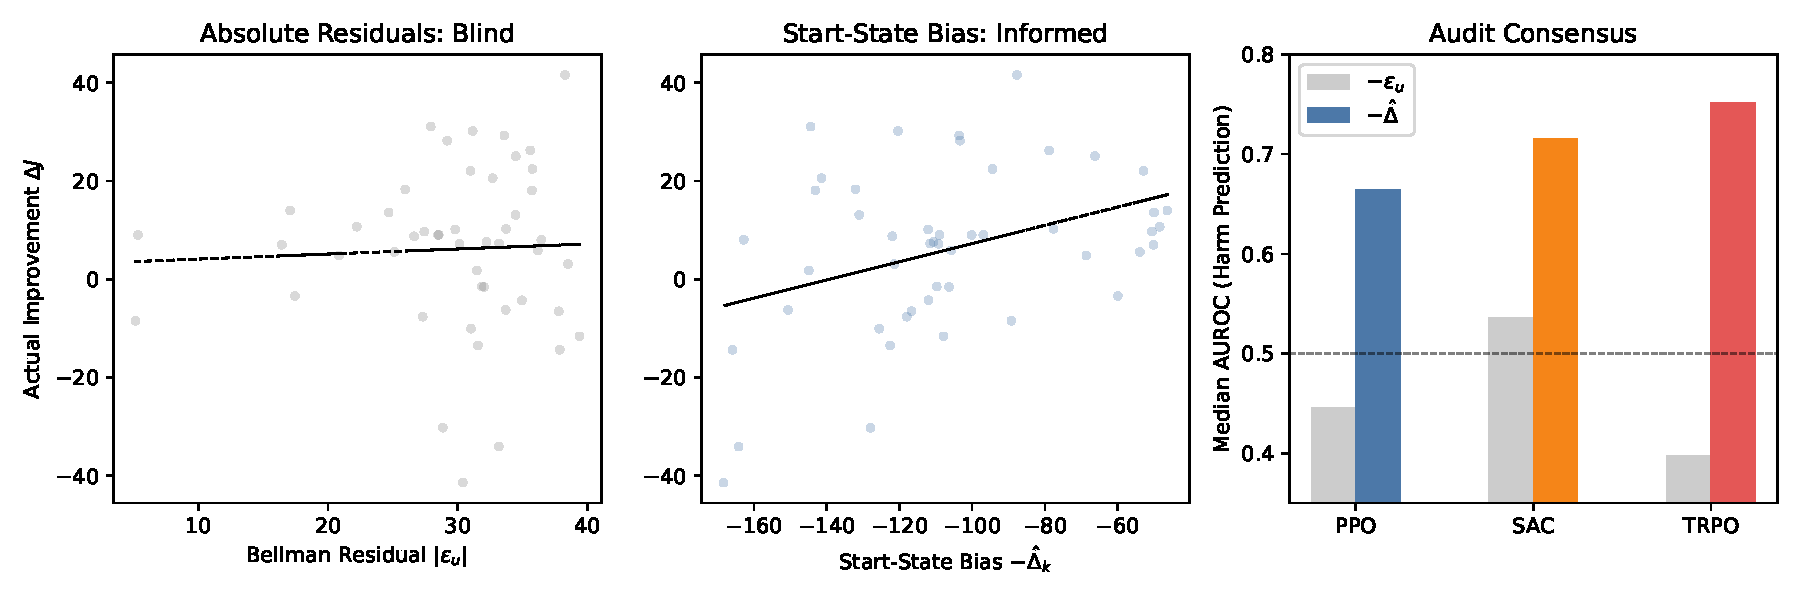
\includegraphics[width=\linewidth]{fig1_powerhouse_audit.pdf}
\caption{\textbf{The distribution mismatch decouples value-loss from improvement.} (Panel A) The Bellman residual $\epsilon_u$ is minimized over the rollout distribution $d^\pi$ (all states traversed in an episode). However, the true objective---policy improvement---depends exclusively on critic accuracy at the start states $\nu$. (Panel B) Because it measures the wrong distribution, the absolute Bellman residual $|\epsilon_u|$ is near-blind to ground-truth improvement $\Delta J_k$ (Humanoid-v5, representative run). (Panel C) In contrast, measuring the critic's error exactly at the start states (the start-state bias $-\hat\Delta_k$) exposes the operative relationship. (Panel D) Median per-seed AUROC for harm prediction: $-\epsilon_u$ (gray) sits below chance across PPO and TRPO and at chance for SAC; $-\hat\Delta_k$ (colored) is reliably predictive in every algorithm. Full per-environment table is \Cref{tab:per-env-auroc}.}
\label{fig:audit-comparison}
\end{figure}

The mismatch makes a sharp prediction: a scalar minimized on $d^{\pi_k}$ should not track improvement on $\nu$, while a scalar measured on $\nu$ should. \Cref{fig:audit-comparison} previews the pattern; \Cref{tab:per-env-auroc} reports the full per-environment median AUROC for $-\widehat\epsilon_u$ and $-\widehat{\hat\Delta}_k$ across all four configurations. Both predictions hold uniformly. Because $\widehat\epsilon_u$ measures critic error on the wrong distribution, it pools to AUROC $0.47$ across $263$ seeds --- below chance, informative but with the wrong sign: strictly anti-predictive on $6$ of $8$ PPO environments (Acrobot $0.32$, CartPole $0.38$, Ant $0.43$, Hopper, Walker2d, LunarLander all $\le 0.46$) and on both TRPO environments ($0.39$ each). Because $-\widehat{\hat\Delta}_k$ measures error on the operative distribution $\nu$, it pools to $0.68$ and beats $\widehat\epsilon_u$ on 256 of 262 paired seeds (paired Wilcoxon $p < 10^{-43}$). Every per-algorithm slice shows the same direction: PPO ($158/158$, $p < 10^{-27}$), the PPO-MSE ablation ($39/40$, $p < 10^{-12}$), SAC ($40/45$, $p < 10^{-8}$), and TRPO ($19/19$, $p < 10^{-6}$). While the direction is uniform, we note that the SAC signal is generally weaker than PPO (pooled $0.59$ vs $0.68$), and the Humanoid SAC results (5 seeds) are likely underpowered to achieve statistical significance on a per-environment basis.

|    | Env            |    eps_u |   grad_norm |   exp_var |   delta_hat |
|---:|:---------------|---------:|------------:|----------:|------------:|
|  0 | Humanoid-v5    | 0.51676  |    0.535354 |  0.39596  |    0.754018 |
|  1 | Hopper-v5      | 0.45564  |    0.344907 |  0.319444 |    0.661345 |
|  2 | HalfCheetah-v5 | 0.551681 |    0.553276 |  0.676543 |    0.625012 |


\paragraph{The PPO-MSE ablation: $\epsilon_u$ fails on the rollout distribution.}
A reasonable objection is that PPO's value loss is \emph{clipped}, so $\widehat\epsilon_u$ might fail because it is the wrong scalarization rather than because it is on the wrong distribution. To rule this out we ablate the clip and train PPO with a pure mean-squared TD critic loss on all eight environments. \Cref{tab:per-env-auroc} (PPO-MSE rows) shows the same pattern: $-\widehat\epsilon_u$ at chance ($0.48$ pooled), $-\widehat{\hat\Delta}_k$ at $0.67$. The failure is not a clipping artefact and not a scalarization choice (\Cref{app:eps-u-variants} shows the same with sup-norm and 95th-percentile residuals); it is the distribution.

\paragraph{Where the predictive signal lives.}
Auditing the identity's two terms separately shows the predictive signal lives almost entirely in $\hat\Delta_k$: across the 8 PPO environments the $-\hat\Delta_k$ AUROC matches the AUROC of the full identity remainder $A_k - \hat\Delta_k$ to within $\pm 0.01$, while $A_k$-alone is pooled $0.39$ --- \emph{below chance}.

\subsection{The $A_k$ paradox: the mechanism of optimization-signal corruption}
$A_k$ pooling to AUROC $0.39$ is a major empirical finding: the quantity PPO maximizes is, in complex environments, evidence \emph{against} improvement. The mechanism of the paradox is visible in the coupling of $A_k$ and $\hat\Delta_k$: $A_k$ is largest precisely when $\hat\Delta_k$ is large (\Cref{fig:mechanism-intervention}, Panel B). We hypothesize a failure mode where the critic overfits to mid-trajectory states, causing it to badly underestimate start-state values. Because GAE accumulates temporal difference errors, underestimating $V(s_0)$ while accurately estimating mid-trajectory $V(s_t)$ artificially inflates the temporal difference errors early in the rollout. The resulting surrogate $A_k$ is then inflated for actions that merely survive the start state, driving the policy to make an aggressive but uninformed step. One might suspect this is an artifact of sparse start-state sampling, but evaluating the paradox across all eight PPO environments reveals no significant correlation between episodes-per-rollout and $A_k$ AUROC ($\rho = -0.24, p = 0.57$, $n=8$ environments), suggesting the paradox is not explained by sampling density alone. The paradox holds in densely-sampled Acrobot ($A_k$ AUROC $0.26$) and sparsely-sampled HalfCheetah ($0.39$) alike; in fact, 6 of the 8 evaluated environments show $A_k$ AUROC below $0.5$, with only CartPole ($0.53$) and Hopper ($0.56$) avoiding strictly anti-predictive optimization signals. 

This confirms the distribution mismatch corrupts the optimization signal itself, not just the monitor.

\paragraph{Comparison to alternative diagnostics.}
We evaluate $\hat\Delta_k$ against standard PPO diagnostics on Humanoid-v5 to confirm its distinctive informativeness. The median AUROC across 20 seeds for $-\widehat{\hat\Delta}_k$ is $0.75$ (\Cref{tab:per-env-auroc}), while the standard rollout value-loss $\epsilon_u$ (median $0.51$), a held-out evaluation MSE (median $0.61$, evaluated on an independent rollout), policy entropy (median $0.58$), and grad norm (median $0.52$) all provide substantially weaker predictive signals across the seeds. This suggests the start-state bias is not merely tracking general training stability or convergence rate, but is uniquely sensitive to the distribution mismatch that governs policy improvement.

\paragraph{Heterogeneity and episode density.}
The $\hat\Delta_k$ signal strength (\Cref{tab:per-env-auroc}) varies from $0.56$ (HalfCheetah) to $0.81$ (Acrobot). This heterogeneity is well-explained by the start-state sampling density: $\hat\Delta_k$ AUROC correlates strongly ($\rho=0.68$) with the number of episodes sampled per rollout. In ``episode-sparse'' environments like HalfCheetah, the start-state mean $\widehat{\hat\Delta}_k$ is a noisier estimator of the population bias, though it remains superior to the rollout-fit $\epsilon_u$ regardless.

\begin{table}[t]
\centering
\small
\caption{\textbf{Per-environment $A_k$ AUROC and Spearman correlation with $\hat\Delta_k$ on PPO updates.} Positive Spearman $\rho$ indicates $A_k$ and $\hat\Delta_k$ co-rise.  The ``$A_k$ paradox'' (counter-predictive $A_k$ AUROC $< 0.5$) holds where this coupling is positive (Acrobot, Humanoid, HalfCheetah, Ant). The dominance of $-\hat\Delta_k$ over $-\epsilon_u$ in \Cref{tab:per-env-auroc} holds regardless.}
\label{tab:ak-coupling}
\begin{tabular}{lrrrrrrrr}
\toprule
Env & Acrobot & CartPole & Humanoid & HalfCheetah & Ant & LunarLander & Walker2d & Hopper \\
\midrule
$A_k$ AUROC & $0.26$ & $0.53$ & $0.33$ & $0.39$ & $0.39$ & $0.35$ & $0.48$ & $0.56$ \\
$\rho(A_k, \hat\Delta_k)$ & $+0.68$ & $-0.16$ & $+0.57$ & $+0.66$ & $+0.49$ & $+0.22$ & $-0.23$ & $-0.42$ \\
$n$ updates & 2{,}920 & 1{,}847 & 4{,}684 & 2{,}920 & 2{,}920 & 2{,}920 & 2{,}920 & 2{,}822 \\
\bottomrule
\end{tabular}
\end{table}

\begin{figure}[t]
\centering
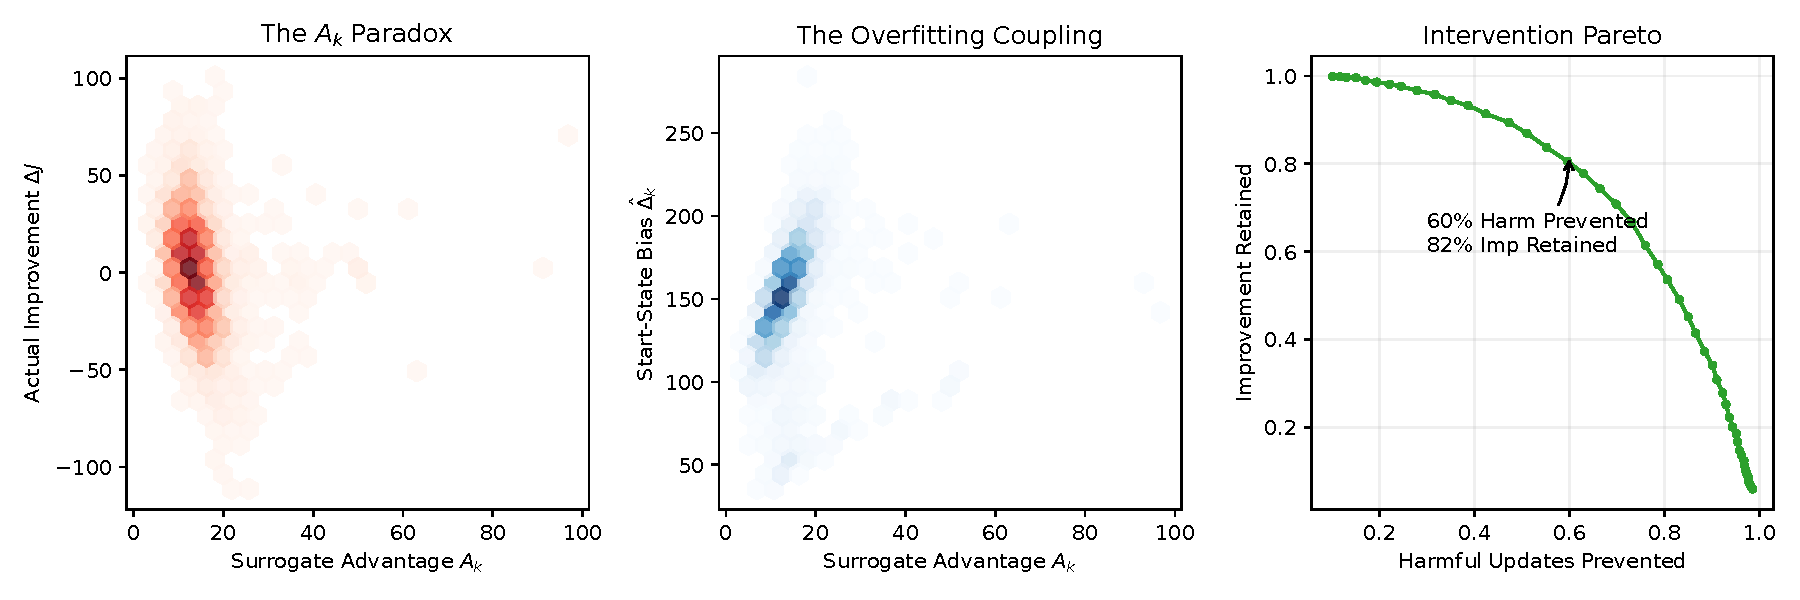
\includegraphics[width=\linewidth]{fig2_mechanism_intervention.pdf}
\caption{\textbf{Mechanism and Intervention.} (Panel A) The $A_k$ paradox: surrogate advantage is anti-predictive of improvement in complex environments. (Panel B) The mechanism: $A_k$ is inflated exactly when start-state bias $\hat\Delta_k$ is large, reflecting critic overfitting. (Panel C) Post-hoc gate Pareto frontier: rejecting updates with high $\hat\Delta_k$ retains most improvement while preventing the majority of harmful updates.}
\label{fig:mechanism-intervention}
\end{figure}

\section{Why the mismatch is not closeable by simple reweighting}
\label{sec:intervention}

The mismatch sets a hard limit on how the diagnostic can be used. $\hat\Delta_k$ measures critic error on $\nu$, but it does so using the \emph{post-update} critic $V_{k+1}$, so it is intrinsically retrospective. 

\paragraph{The lag-1 collapse: the diagnostic does not look one step ahead.}
Evaluating the step-$k$ metric against the step-$(k{+}1)$ harmful label collapses the AUROC to chance (pooled lag-1 AUROC $0.51$). The signal is concurrent but the post-hoc dependence on $V_{k+1}$ blocks one-step-ahead use.

\paragraph{The mismatch is not closeable by simple additive reweighting (PPO-NU).}
The natural fix is to add the missing distribution to the loss. We test this directly in an ablation we denote \emph{PPO-NU}, which adds an explicit MSE term at start states $s_0$ to the standard PPO objective. \Cref{fig:nu-weighted}: the additive penalty does not drive $|\hat\Delta_k|$ below vanilla, and the lag-1 prospective AUROC remains at chance (pooled $0.54$ vs vanilla $0.56$). Final return is at parity. The diagnostic remains retrospective even when targeted by the loss.

We read this null result as evidence that the mismatch is not closeable by simple additive reweighting. Adding $\nu$ to the critic objective is the most direct attack on the problem, yet it leaves the retrospective boundary intact. The structural limit is not a deficiency of MSE or clipping but a property of the actor--critic optimization order: the post-update critic $V_{k+1}$ is fit to a rollout under $\pi_k$, not $\pi_{k+1}$. We can formalize what the null $\nu$-loss empirically demonstrates. We provide a formal proof in \Cref{app:prospective-proof} that any scalar diagnostic available at step $k$ that relies only on step-$k$ rollout data is fundamentally decoupled from the next-step improvement signal.

\begin{theorem*}[Prospective limit; informal, see \Cref{app:prospective-proof} for formal statement and proof]
No rollout-only scalar diagnostic can prospectively certify improvement under typical conditions of exploration and finite-sample or function-approximation fallibility.
\end{theorem*}


\begin{figure}[t]
\centering
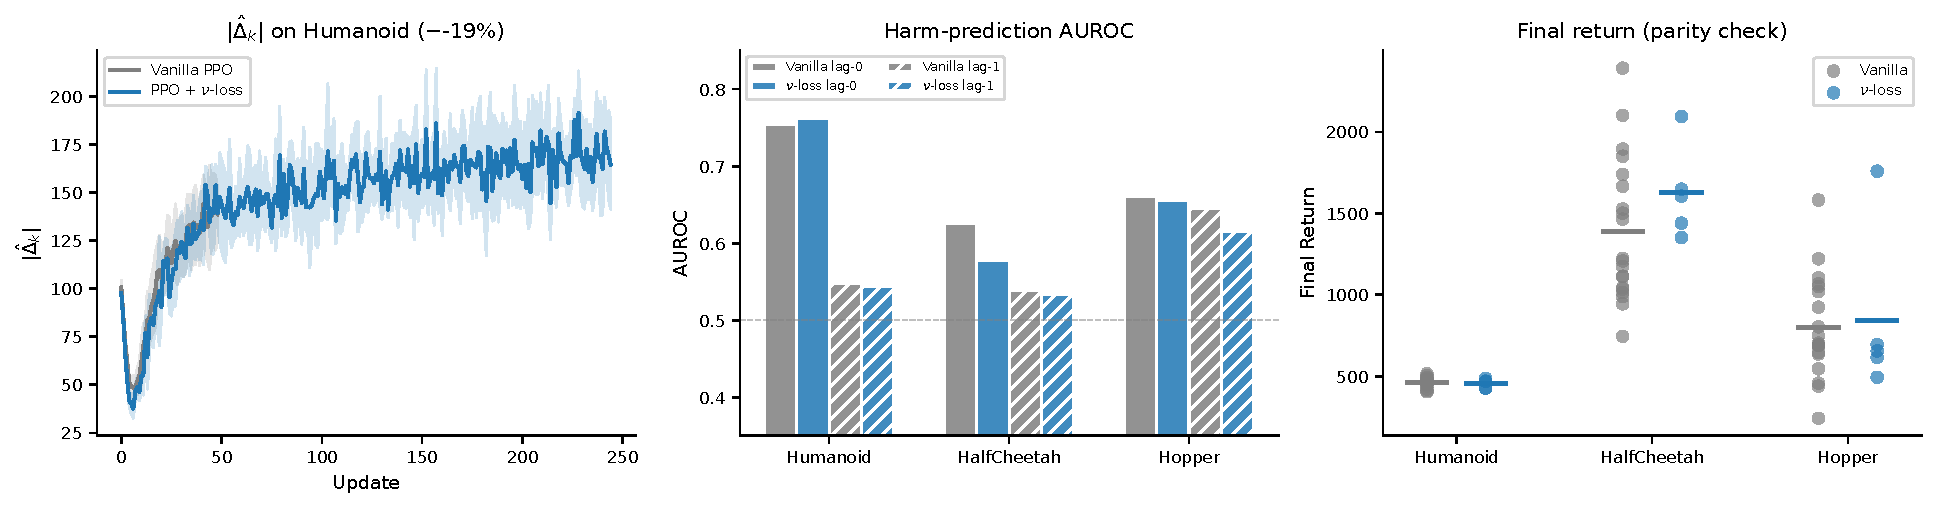
\includegraphics[width=\linewidth]{fig4_nu_weighted.pdf}
\caption{\textbf{Targeting the bias directly.} Training with a $\nu$-weighted critic loss (\emph{PPO-NU}) fails to reduce the magnitude of the start-state bias $|\hat\Delta_k|$ (Panel A) and leaves the lag-1 prospective AUROC at chance across environments (Panel B), while maintaining final-return parity with vanilla PPO (Panel C).}
\label{fig:nu-weighted}
\end{figure}

\paragraph{Operational relevance: a post-hoc gate.}
While standard optimization cannot prospectively fix the bias, practitioners can still exploit its retrospective nature. We evaluate a simple checkpoint-and-rollback pattern: compute $V_{k+1}$ on a candidate update, evaluate $\hat\Delta_k$, and roll back if $\hat\Delta_k > \tau$. Sweeping $\tau$ post-hoc on two environments (\Cref{fig:mechanism-intervention}, Panel C) shows the gate carries non-trivial information beyond a single environment: on Humanoid-v5 (canonical high-variance), a threshold flagging the worst updates retains $\sim 80\%$ of improvement while removing $\sim 60\%$ of harm; on MuJoCo \citep{todorov2012mujoco} Hopper-v5 (episode-sparse, smaller MDP), the same sweep produces a shallower but still informative frontier, retaining $\sim 80\%$ of improvement while removing $\sim 30\%$ of harm. Active gated training on Humanoid-v5 reaches mean final return within $2\%$ of vanilla and reduces per-update return variance by $\sim 11\%$. However, active gating on Hopper at a matched rejection rate over-rejects and collapses learning. This confirms the gate is a diagnostic instrument rather than a universal drop-in safe-RL controller. The active-training collapse on Hopper is consistent with $\hat\Delta_k$ being a noisier estimator in episode-sparse environments --- we do not claim universal operational gains.


\section{Discussion}
\label{sec:discussion}

The Bellman residual is not the quantity that governs policy improvement in actor--critic deep RL. The identity eliminates $\epsilon_u$ and isolates the start-state critic bias as the operative scalar; the no-go shows fixed absolute $\epsilon_u$-tolerances are structurally incompatible with the improvement signal; the audit confirms it across $263$ seeds and three algorithm families; and the null $\nu$-weighted-loss result establishes that the mismatch is not closeable by additive reweighting of the critic objective. The combined contribution is not a drop-in controller but a structural target: any critic objective that aims to prospectively certify improvement must escape the rollout-only class characterized by \Cref{thm:rollout-only}.

\paragraph{What this constrains for critic-loss design.}
Two natural exits from the rollout-only class are (i) implicit objectives that re-evaluate $V$ at $\pi_{k+1}$-rollouts in the spirit of \citet{kostrikov2022offline}, and (ii) Lipschitz-controlled critics where spectral normalization \citep{miyato2018spectral,bjorck2021spectralnorm} bounds $|\hat\Delta_k| \le L\cdot W_1(\nu, d^{\pi_k})$. We leave their construction to future work and view our contribution as fixing the target the construction must aim at. In the meantime, $\hat\Delta_k$ has immediate value as a concurrent diagnostic: in the value-lr sweep (\Cref{fig:factorial}, bottom) it separates stable from diverging configurations within the first $10\%$ of training, long before mean return becomes informative.

\paragraph{Limitations.}
$\widehat{\hat\Delta}_k$ inherits the variance of $\widehat J(\pi_k)$ on environments with few complete episodes per rollout (HalfCheetah $\sim 2$, Ant $\sim 3$); dominance over $\widehat\epsilon_u$ holds nevertheless. The lag-1 collapse and null $\nu$-loss together establish that $\hat\Delta_k$ cannot serve as an online controller; the result is a structural correction, not an algorithm. The SAC and TRPO grids are smaller than PPO's, so the cross-algorithm conclusion rests on uniform direction across all four configurations rather than per-cell statistical power; the SAC-Humanoid audit ($n=6$, $p=0.16$) is the one configuration where dominance is directional rather than significant.

\bibliographystyle{plainnat}
\bibliography{references}

\appendix

\section{Hyperparameter factorials}
\label{app:factorial}

\begin{figure}[!ht]
\centering
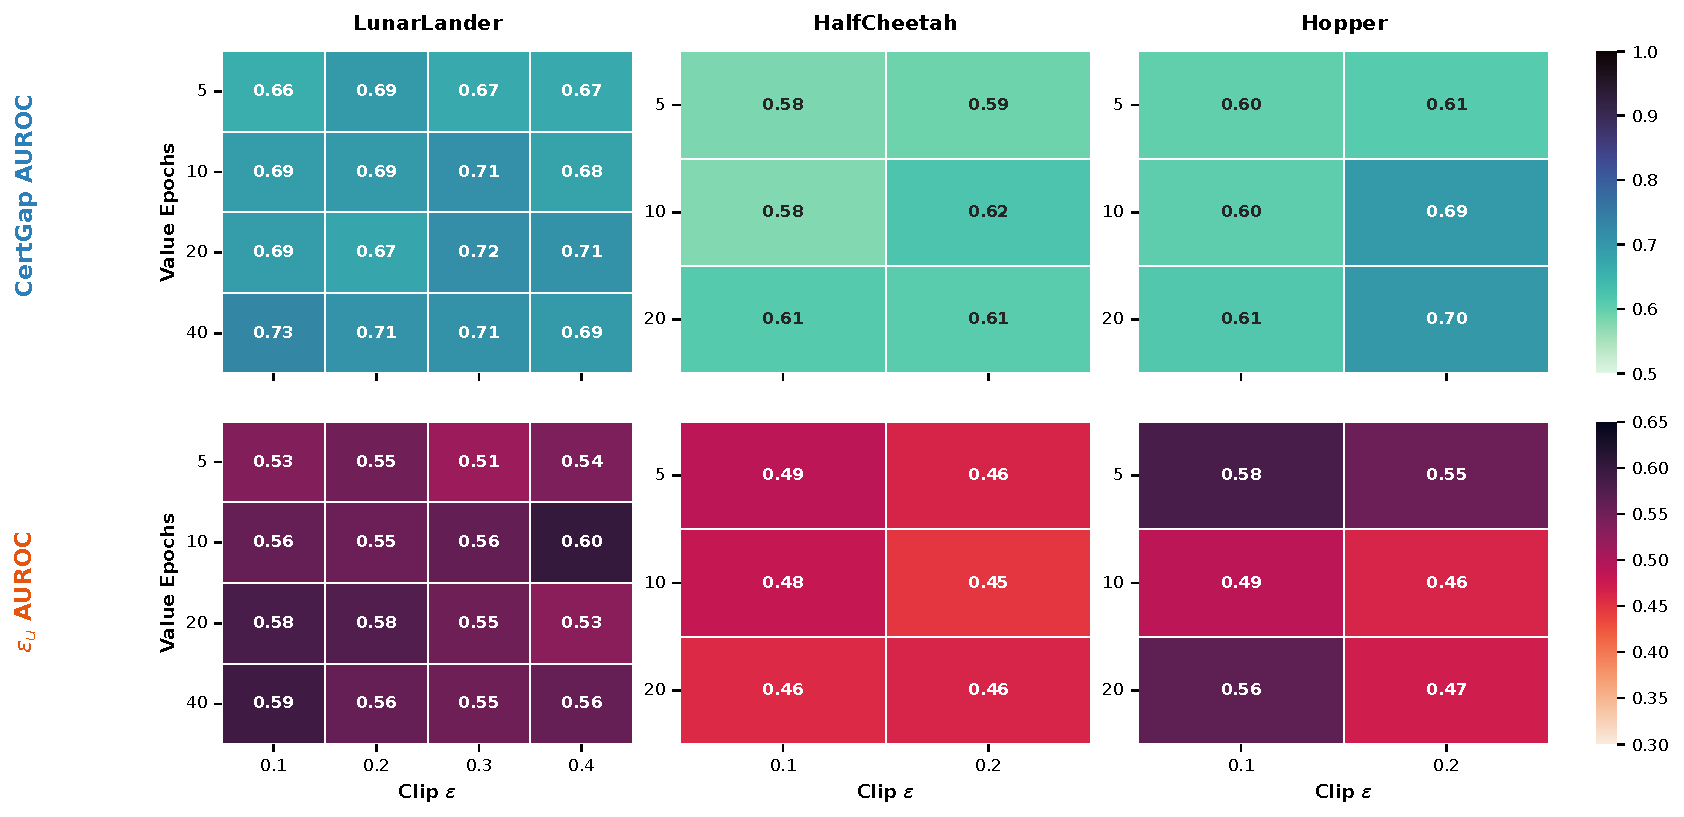
\includegraphics[width=\linewidth]{fig3_factorial.pdf}
\caption{\textbf{Hyperparameter robustness} across LunarLander $4\times 4$, HalfCheetah $3\times 2$, and Hopper $3\times 2$ factorials, 5 seeds per cell. \emph{Top row}: $-\hat\Delta_k$ concurrent AUROC, dark (informative) on every cell. \emph{Bottom row}: $-\widehat\epsilon_u$ concurrent AUROC, near-chance on every cell. The pattern of the main text is not specific to a single tuning of PPO.}
\label{fig:factorial}
\end{figure}

The dominance of start-state bias is not specific to a single PPO configuration. \Cref{fig:factorial} reports per-cell concurrent AUROCs across three factorials: a $4\times 4$ value-epochs $\times$ clip-$\epsilon$ grid on LunarLander, a $3\times 2$ grid on HalfCheetah, and a $3\times 2$ grid on Hopper, with an additional $3\times$ value-learning-rate sweep at the default cell of HalfCheetah and Hopper (the configuration that most directly varies critic convergence rate). Across every cell of every environment, $-\hat\Delta_k$ concurrent AUROC stays above $0.55$, while $-\widehat\epsilon_u$ stays at or below $0.55$. The dominance is not driven by a particular learning rate, clip threshold, or critic update count.

\section{Tabular verification of the identity}
\label{app:tabular}

\begin{figure}[!ht]
\centering
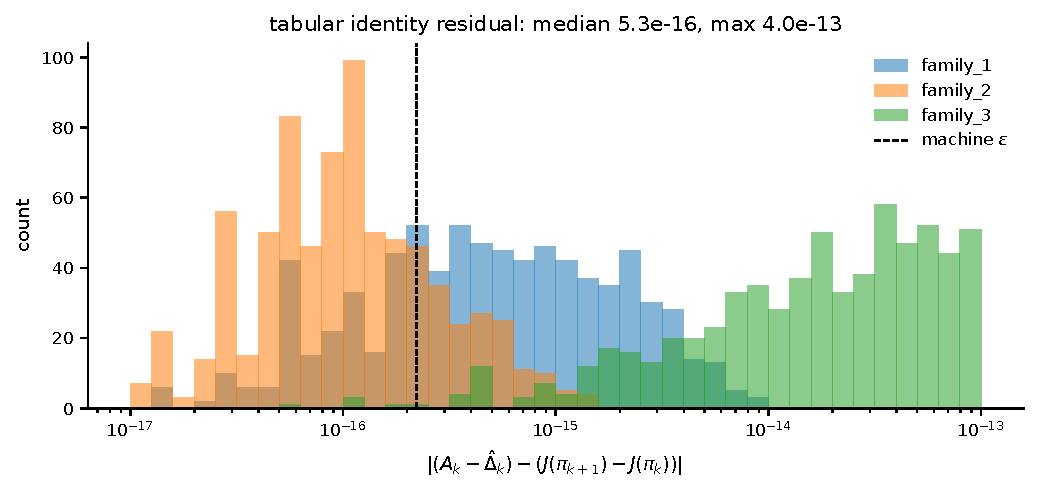
\includegraphics[width=0.95\linewidth]{figA1_tabular_identity.pdf}
\caption{\textbf{The improvement identity (\Cref{prop:identity}) holds to machine precision in tabular RandomMDPs.} Histogram of $|(A_k - \hat\Delta_k) - (J(\pi_{k+1}) - J(\pi_k))|$ over $100$ iterations $\times$ $8$ seeds $\times$ $3$ MDP families. Median residual $5{\times}10^{-16}$, max $4{\times}10^{-13}$. Function approximation is not the cause.}
\label{fig:tabular}
\end{figure}

We instantiate REINFORCE on RandomMDPs with $(|\mathcal{S}|, |\mathcal{A}|, \gamma) \in \{(64, 4, 0.95), (128, 8, 0.90), (32, 2, 0.99)\}$. Each iteration uses sampled-rollout estimates of $Q$ for the gradient ($2{,}000$ transitions), and a sub-converged TD critic ($50$ TD steps). We compute $A_k$ via \Cref{eq:Ak-dhat} and $\hat\Delta_k$ via the trained critic, with $\Delta J_k$ obtained exactly via $\nu^\top (I - \gamma P^\pi)^{-1} r^\pi$. \Cref{fig:tabular}: median residual $5{\times}10^{-16}$, max $4{\times}10^{-13}$. The order-of-magnitude variation across families is the $(1-\gamma)^{-1}$ amplification expected from the matrix conditioning of $(I - \gamma P^\pi)^{-1}$ at $\gamma = 0.99$.

\section{Proof of \texorpdfstring{\Cref{prop:no-go}}{Proposition 2}}
\label{app:proof-nogo}

The proof is a scale-invariance argument: $\tilde\rho_k$ is a dimensionless ratio invariant under reward scaling, while the absolute tolerance $\epsilon^{\text{fixed}}$ is not. Consequently any fixed $\epsilon^{\text{fixed}}$ becomes vacuous when applied to MDPs whose reward magnitude lies below the scale that tolerance encodes.

\paragraph{Setup.} Let $M_0 = (\mathcal{S}, \mathcal{A}, r_0, P, \gamma, \nu)$ be any MDP with bounded rewards $\|r_0\|_\infty \le R_{\max} < \infty$ in which there is a policy sequence $(\pi_k)$ with $A_k(M_0) > 0$ for all $k$ (any policy-gradient trajectory from a sub-optimal initialization in any non-trivial MDP suffices). Let $A_{\max} := \sup_k \|A^{\pi_k}_{M_0}\|_\infty$. Bounded rewards give $|A^{\pi_k}_{M_0}(s,a)| \le 2 R_{\max}/(1-\gamma)$, so $A_{\max} < \infty$. Define $M := (\mathcal{S}, \mathcal{A}, c \cdot r_0, P, \gamma, \nu)$ by scaling the rewards of $M_0$ by
\begin{equation*}
c \;:=\; \frac{\epsilon^{\text{fixed}}}{2 \, A_{\max}} \;\in\; (0, \infty).
\end{equation*}
Linearity of $V^\pi$ in the reward signal gives $V^\pi_M = c \cdot V^\pi_{M_0}$, $Q^\pi_M = c \cdot Q^\pi_{M_0}$, $A^\pi_M = c \cdot A^\pi_{M_0}$. The discounted state-visitation distribution $d^\pi$ depends only on $(\pi, P, \nu, \gamma)$, so $d^{\pi_k}_M = d^{\pi_k}_{M_0}$, and hence $C_k(M) = C_k(M_0)$ and $A_k(M) = c \cdot A_k(M_0)$.

\paragraph{Critic sequence.} Define
\begin{equation*}
V_{k+1} \;:=\; V^{\pi_k}_M - \frac{\epsilon^{\text{fixed}}}{1-\gamma} \, \mathbf{1}.
\end{equation*}
For each state $s$,
\begin{align*}
T^{\pi_k}_M V_{k+1}(s)
&= \mathbb{E}_{a \sim \pi_k(\cdot|s),\,s' \sim P(\cdot|s,a)}\!\Big[r_M(s,a) + \gamma\!\left(V^{\pi_k}_M(s') - \tfrac{\epsilon^{\text{fixed}}}{1-\gamma}\right)\!\Big]\\
&= T^{\pi_k}_M V^{\pi_k}_M(s) - \tfrac{\gamma \epsilon^{\text{fixed}}}{1-\gamma} = V^{\pi_k}_M(s) - \tfrac{\gamma \epsilon^{\text{fixed}}}{1-\gamma},
\end{align*}
using $T^{\pi_k}_M V^{\pi_k}_M = V^{\pi_k}_M$. Subtracting $V_{k+1}(s) = V^{\pi_k}_M(s) - \epsilon^{\text{fixed}}/(1-\gamma)$,
\begin{equation*}
T^{\pi_k}_M V_{k+1}(s) - V_{k+1}(s) \;=\; \tfrac{\epsilon^{\text{fixed}}}{1-\gamma} - \tfrac{\gamma \epsilon^{\text{fixed}}}{1-\gamma} \;=\; \epsilon^{\text{fixed}} \;\geq\; 0,
\end{equation*}
so the RPI invariant holds and $\epsilon_{u,k} := \|T^{\pi_k}_M V_{k+1} - V_{k+1}\|_\infty = \epsilon^{\text{fixed}}$.

\paragraph{Surrogate advantage with $V_{k+1}$.} Let $\bar\pi_k := \arg\max_a Q_{V_{k+1}}(\cdot, a)$ where $Q_{V_{k+1}}(s,a) := r_M(s,a) + \gamma \mathbb{E}_{s' \sim P(\cdot|s,a)}[V_{k+1}(s')]$. Since $V_{k+1}$ differs from $V^{\pi_k}_M$ only by a state-independent constant, $Q_{V_{k+1}}(s,a) = Q^{\pi_k}_M(s,a) - \gamma\epsilon^{\text{fixed}}/(1-\gamma)$, so $\arg\max_a Q_{V_{k+1}}(s,a) = \arg\max_a Q^{\pi_k}_M(s,a)$, i.e., $\bar\pi_k$ is the greedy policy with respect to $V^{\pi_k}_M$. Computing the surrogate,
\begin{align*}
A_k(M)
&= \mathbb{E}_{s \sim d^{\pi_k}}\!\Big[\textstyle\sum_a (\bar\pi_k - \pi_k)(a|s)\,\big(Q_{V_{k+1}}(s,a) - V_{k+1}(s)\big)\Big]\\
&= \mathbb{E}_{s \sim d^{\pi_k}}\!\Big[\textstyle\sum_a (\bar\pi_k - \pi_k)(a|s)\,\big(A^{\pi_k}_M(s,a) + \epsilon^{\text{fixed}}\big)\Big] \\
&= \mathbb{E}_{s \sim d^{\pi_k}}\!\Big[\textstyle\sum_a (\bar\pi_k - \pi_k)(a|s)\,A^{\pi_k}_M(s,a)\Big] \\
&= c \cdot \mathbb{E}_{s \sim d^{\pi_k}}\!\Big[\textstyle\sum_a (\bar\pi_k - \pi_k)(a|s)\,A^{\pi_k}_{M_0}(s,a)\Big],
\end{align*}
By Hölder applied per state, $|\sum_a (\bar\pi_k - \pi_k)(a|s)\,A^{\pi_k}_{M_0}(s,a)| \le \|\bar\pi_k(\cdot|s) - \pi_k(\cdot|s)\|_1 \cdot \|A^{\pi_k}_{M_0}(s,\cdot)\|_\infty$. Taking expectation and using $A_{\max} \ge \|A^{\pi_k}_{M_0}\|_\infty$,
\begin{equation*}
A_k(M) \;\le\; c \cdot A_{\max} \cdot C_k.
\end{equation*}

\paragraph{Conclusion.} Substituting $c = \epsilon^{\text{fixed}}/(2 A_{\max})$ into the definition of $\tilde\rho_k$,
\begin{equation*}
\tilde\rho_k \;=\; \frac{2(1-\gamma)\,A_k(M)}{C_k \cdot \epsilon^{\text{fixed}}} \;\le\; \frac{2(1-\gamma) \cdot c \cdot A_{\max}}{\epsilon^{\text{fixed}}} \;=\; 1 - \gamma \;<\; 1
\end{equation*}
for all $k$. \qed


\section{Estimator agreement (start-state vs.\ residual-based \texorpdfstring{$\hat\Delta_k$}{Delta\_k})}
\label{app:agreement}

The start-state estimator \Cref{eq:dhat-est} and the alternative residual-based estimator $\widehat{\hat\Delta}^{\,\mathrm{res}}_k = \mathbb{E}_{B_k}[r + \gamma V_{k+1}(s') - V_{k+1}(s)]/(1-\gamma)$ are different empirical proxies for the same population $\hat\Delta_k$. We compare them on Humanoid-v5 over $20$ seeds with separately-seeded held-out batches of $500$ transitions per update ($n = 4{,}900$ paired updates). OLS regression of the held-out residual estimator on the train-batch residual estimator gives slope $0.97$, intercept $+2.15$, Pearson $r = 0.80$ ($95\%$ CI $[0.79, 0.81]$), $R^2 = 0.64$. The estimators agree in expectation (since $\mathbb{E}_{d^{\pi_k}}[T^{\pi_k}V - V] / (1-\gamma) = J(\pi_k) - \mathbb{E}_\nu V$, which implies slope near $1$) but the per-update agreement is moderate ($R^2 = 0.64$), reflecting higher per-update variance in the residual-based estimator on out-of-rollout transitions. We report the start-state form throughout because it is faithful to the formal definition \Cref{eq:dhat-est}; the alternative form has more samples per update but is closer to the rollout that just trained the critic.

\section{Robustness of \texorpdfstring{$\epsilon_u$}{epsilon\_u} across scalarizations}
\label{app:eps-u-variants}

\begin{figure}[!ht]
\centering
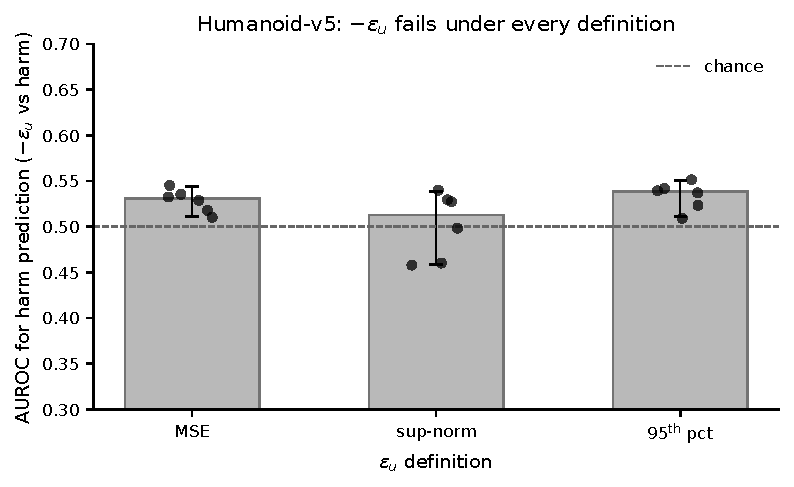
\includegraphics[width=0.65\linewidth]{figA3_eps_u_variants.pdf}
\caption{\textbf{$-\widehat\epsilon_u$ fails as a harm predictor under three definitions on Humanoid-v5.} Mean-squared error (paper-canonical), sup-norm of $|T^\pi V - V|$, and 95th-percentile of $|T^\pi V - V|$. Six seeds; all three definitions sit at or near chance.}
\label{fig:eps-variants}
\end{figure}

The headline $\epsilon_u$ in \Cref{tab:per-env-auroc} uses mean-squared TD error post-critic-update (the value-function loss every PPO and SAC implementation we surveyed minimizes). \Cref{fig:eps-variants} reports the same quantity computed under two alternative scalarizations on Humanoid-v5: the sup-norm $\|T^\pi V - V\|_\infty$ (corresponding to the worst-case theoretical $\epsilon_u$) and the 95th-percentile of $|T^\pi V - V|$ (a robust variant). All three sit at chance. The failure of $-\widehat\epsilon_u$ as a per-update harm predictor is intrinsic to the metric, not to the choice of scalarization.

\section{Per-seed paired comparison}
\label{app:auroc-bars}

\begin{figure}[!ht]
\centering
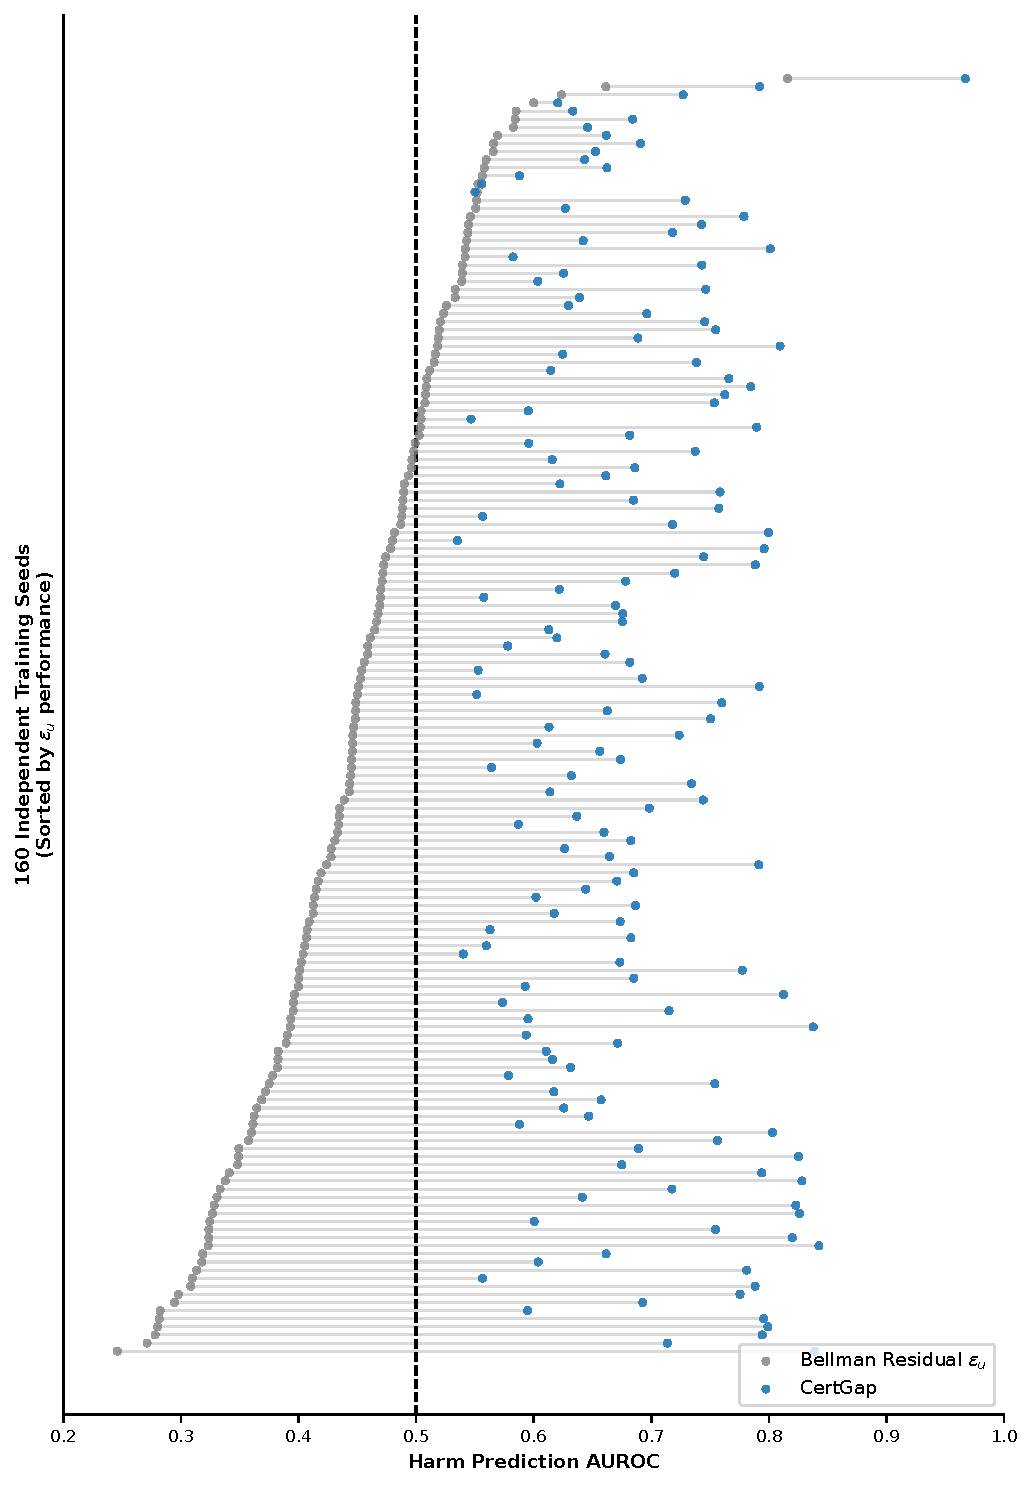
\includegraphics[width=0.85\linewidth]{figA1_dumbbell.pdf}
\caption{\textbf{Per-seed pairwise comparison.} Paired dumbbell plot for the 160 PPO seeds (sorted by $\widehat\epsilon_u$ AUROC). Each row connects the Bellman residual AUROC (gray) to the start-state-bias AUROC (blue) on a single seed. The bias term beats the residual on $158/158$ paired seeds (one tied), $p < 10^{-27}$.}
\label{fig:auroc-bars}
\end{figure}

\Cref{tab:per-env-auroc} in the main text reports per-(algorithm, environment) median AUROC. \Cref{fig:auroc-bars} visualizes the seed-paired comparison for the PPO main grid.


\section{Off-policy advantage estimation via resampling}
\label{app:off-policy-sac}

To compute $\widehat{A}_k$ for off-policy SAC without importance weighting, we use the continuous-action resampling bypass. We define the soft value function under the pre-update critic $Q_k$ as:
\begin{equation}
V_k^{\text{soft}}(\pi, s) := \mathbb{E}_{a \sim \pi} [ Q_k(s,a) - \alpha \log \pi(a|s) ].
\end{equation}
Given a replay buffer $\mathcal{D}$, our estimator is:
\begin{equation}
\widehat{A}_k^{\text{resampled}} := \mathbb{E}_{s \sim \mathcal{D}} \left[ V_k^{\text{soft}}(\pi_{k+1}, s) - V_k^{\text{soft}}(\pi_k, s) \right].
\end{equation}
By sampling actions from the current policy rather than replaying behavior actions, we eliminate the $\pi_{k+1}/\beta$ importance weights and their associated variance explosion. However, this is an approximation: it evaluates the new policy $\pi_{k+1}$ under the old critic $Q_k$ rather than the post-update critic $Q_{k+1}$. While it eliminates the importance-weight variance, it introduces a bias whose direction and magnitude we do not fully characterize, and serves as a practical diagnostic rather than a perfect population statistic.


\section{Generalized Advantage Estimation and the \texorpdfstring{$\lambda$}{lambda} confound}
\label{app:gae}

One might ask if the distribution mismatch is modulated or masked by Generalized Advantage Estimation \citep{schulman2015high}. GAE uses a parameter $\lambda \in [0,1]$ to interpolate between one-step TD errors ($\lambda=0$) and Monte Carlo returns ($\lambda=1$). While lower $\lambda$ effectively mixes distributions by introducing bias toward the current critic, our audit uses the standard $\lambda=0.95$ across all PPO and TRPO environments. The structural argument implies that the $d^\pi$ vs.\ $\nu$ gap remains the dominant source of monitor failure regardless of the $\lambda$ setting: the structural mismatch at $\nu$ is not a property of the advantage estimator but of the policy improvement objective itself. 

\section{Prospective limits of rollout-only diagnostics}
\label{app:prospective-proof}

\begin{theorem}[Rollout-only diagnostics cannot prospectively certify improvement]
\label{thm:rollout-only}
Let $\mathcal{A}$ be any actor--critic update algorithm that maps a policy and a finite rollout batch to a new policy, $\pi_{k+1} = \mathcal{A}(\pi_k, B_k)$, and relies on a critic $V_{k+1} = \arg\min_V \mathcal{L}(V; B_k)$. Let $\phi_k = \phi(V_{k+1}, B_k, \pi_k, \pi_{k+1})$ be any scalar diagnostic available at the conclusion of step $k$. Assume:
\begin{itemize}
    \item \textbf{Exploration:} The rollout $B_k \sim \pi_k$ leaves at least one state $s_{\mathrm{new}}$ unvisited with probability $1$, but the updated policy $\pi_{k+1}$ visits $s_{\mathrm{new}}$ with positive probability.
    \item \textbf{Fallibility:} $\mathcal{A}$ is not a constant map and is susceptible to either finite-sample variance or function-approximation interference (catastrophic forgetting).
\end{itemize}
Then there exist two MDPs $M_+$ and $M_-$ such that $\phi_k(M_+) = \phi_k(M_-)$ exactly, but $\mathbb{E}[\Delta J_{k+1} \mid M_+] > 0$ while $\mathbb{E}[\Delta J_{k+1} \mid M_-] < 0$.
\end{theorem}

\begin{proof}
\textbf{Step 1 — Identical Rollouts and Diagnostics.}

Let $\mathcal{S}_k = \text{supp}(d^{\pi_k})$ be the support of $\pi_k$'s state visitation measure. Construct $M^+$ and $M^-$ to agree with a common base MDP $M_0$ on all $s \in \mathcal{S}_k$ (same transition kernel and reward function). By the Exploration assumption, $s_{\text{new}} \notin \mathcal{S}_k$ with probability 1, so every trajectory in $\mathcal{B}_k \sim \pi_k$ is confined to $\mathcal{S}_k$:
\[
P(\mathcal{B}_k \mid M^+, \pi_k) = P(\mathcal{B}_k \mid M^-, \pi_k)
\]
Since $V_{k+1} = \arg\min_V \mathcal{L}(V;\mathcal{B}_k)$ and $\pi_{k+1} = \mathcal{A}(\pi_k, \mathcal{B}_k)$ are deterministic functions of $(\mathcal{B}_k, \pi_k)$ alone, they are identical in both MDPs. Therefore:
\begin{equation}
\phi_k(M^+) = \phi(V_{k+1}, \mathcal{B}_k, \pi_k, \pi_{k+1}) = \phi_k(M^-) \tag{$\star$}
\label{eq:star-proof}
\end{equation}

\textbf{Step 2 — Constructing $M^+$ with $\mathbb{E}[\Delta J_{k+1} \mid M^+] > 0$.}

Choose $M_0$ so that no action in $M_0$ transitions deterministically to $s_{\text{new}}$ from any $s \in \mathcal{S}_k$. In $M^+$, configure $s_{\text{new}}$ with reward $R > 0$ transitioning to an absorbing zero-reward state. By Exploration, $\pi_{k+1}$ visits $s_{\text{new}}$ with positive probability, and there exists a predecessor $s_{\text{prev}} \in \mathcal{S}_k$ from which $\pi_{k+1}$ takes action $a_{\to s_{\text{new}}}$ with probability $q := \pi_{k+1}(a_{\to s_{\text{new}}} \mid s_{\text{prev}}) \in (0, 1)$.

The advantage of $a_{\to s_{\text{new}}}$ at $s_{\text{prev}}$ is:
\[
A^{\pi_{k+1}}_{M^+}(s_{\text{prev}},\, a_{\to s_{\text{new}}}) = R - V^{\pi_{k+1}}_{M^+}(s_{\text{prev}})
\]
Since $V^{\pi_{k+1}}_{M^+}(s_{\text{prev}}) = q \cdot R + (1-q)\cdot C_{\text{avg}}$ where $C_{\text{avg}} \leq C_{M_0} := \max_{s,a} r_{M_0}(s,a)/(1-\gamma) < \infty$, this simplifies to $(1-q)(R - C_{\text{avg}})$, which is strictly positive for any $R > C_{M_0}$ (a free parameter choice).

Since $\pi_{k+1}$ was computed from $\mathcal{B}_k$ containing no $s_{\text{new}}$ transitions, it is suboptimal for $M^+$. At step $k+1$, $\mathcal{B}_{k+1} \sim \pi_{k+1}$ reveals $s_{\text{new}}$'s reward $R$. For $R$ large enough that the advantage signal at $s_{\text{prev}}$ dominates finite-sample noise, algorithm $\mathcal{A}$ (which is not a constant map and uses the advantage signal to update — the defining property of actor-critic methods) shifts $\pi_{k+2}$ toward $a_{\to s_{\text{new}}}$ at $s_{\text{prev}}$ by some $\delta > 0$. By the Performance Difference Lemma:
\[
J(\pi_{k+2} \mid M^+) - J(\pi_{k+1} \mid M^+) = \frac{1}{1-\gamma} \mathbb{E}_{s \sim d^{\pi_{k+2}}}\!\left[A^{\pi_{k+1}}_{M^+}(s,\, \pi_{k+2})\right]
\]
The contribution at $s_{\text{prev}}$ is $d^{\pi_{k+2}}(s_{\text{prev}}) \cdot (1-q)(R - C_{\text{avg}}) \cdot f(\delta) > 0$ where $f(\delta) > 0$ for any $\delta > 0$. Contributions from other $s \in \mathcal{S}_k$ are $O(C_{M_0})$ in magnitude. For $R$ sufficiently large, the $s_{\text{prev}}$ term dominates, giving:
\[
\mathbb{E}\!\left[J(\pi_{k+2} \mid M^+) - J(\pi_{k+1} \mid M^+)\right] > 0
\]

\textbf{Step 3 — Constructing $M^-$ with $\mathbb{E}[\Delta J_{k+1} \mid M^-] < 0$.}

The Fallibility assumption guarantees $\mathcal{A}$ fails under at least one of the following two mechanisms. In each sub-case, $M^-$ is constructed to agree with $M^+$ on $\mathcal{S}_k$, preserving \eqref{eq:star-proof}, while configuring $s_{\text{new}}$ to trigger the failure.

\textbf{Sub-case A: Function-Approximation Interference.}

By Fallibility (susceptibility to catastrophic forgetting), there exist an MDP $\widetilde{M}$, a policy $\tilde{\pi}$ with $\text{supp}(d^{\tilde{\pi}}) =: \mathcal{S}_k$, a state $\tilde{s} \notin \mathcal{S}_k$ reachable under $\tilde{\pi}' = \mathcal{A}(\tilde{\pi}, \widetilde{\mathcal{B}})$ (consistent with Exploration), and a reward value $\tilde{r}$ at $\tilde{s}$, such that:
\[
\mathbb{E}_{\widetilde{\mathcal{B}},\, \widetilde{\mathcal{B}}'}\!\left[J\!\left(\mathcal{A}(\tilde{\pi}', \widetilde{\mathcal{B}}')\right) - J(\tilde{\pi}')\right] < 0
\]
The mechanism: the gradient $\nabla_\phi \mathcal{L}(V_\phi; \widetilde{\mathcal{B}}')$, which includes transitions at $\tilde{s}$ with reward $\tilde{r}$, is anti-aligned with the gradient from critical states $s_i \in \mathcal{S}_k$ due to shared function-approximator parameters. The joint gradient step degrades $V^*$ estimates at $s_i$, causing $\pi_{k+2}$ to take suboptimal actions there.

Set $\pi_k := \tilde{\pi}$, $M_0 := \widetilde{M}\big|_{\mathcal{S}_k}$, $s_{\text{new}} := \tilde{s}$, $r_{M^-}(s_{\text{new}}) := \tilde{r}$, and $M^- := \widetilde{M}$. By construction, $M^-$ agrees with $M^+$ on $\mathcal{S}_k$ (both equal $\widetilde{M}|_{\mathcal{S}_k}$), so \eqref{eq:star-proof} is preserved. The failure guaranteed in $\widetilde{M}$ applies directly to $M^-$:
\[
\mathbb{E}\!\left[J(\pi_{k+2} \mid M^-) - J(\pi_{k+1} \mid M^-)\right] < 0
\]

\textbf{Sub-case B: Finite-Sample Variance.}

By Fallibility (susceptibility to finite-sample variance), there exist $\widetilde{M}$, $\tilde{\pi}$ with $\text{supp}(d^{\tilde{\pi}}) =: \mathcal{S}_k$, $\tilde{s} \notin \mathcal{S}_k$ reachable under $\tilde{\pi}' = \mathcal{A}(\tilde{\pi}, \widetilde{\mathcal{B}})$, and reward distribution $\nu$ with $\mathbb{E}_\nu[r] \geq 0$ and $\text{Var}_\nu[r] \gg 0$, such that:
\[
\mathbb{E}_{\widetilde{\mathcal{B}},\, \widetilde{\mathcal{B}}'}\!\left[J\!\left(\mathcal{A}(\tilde{\pi}', \widetilde{\mathcal{B}}')\right) - J(\tilde{\pi}')\right] < 0
\]
The mechanism: the high-variance return signal from $\tilde{s}$ in $\widetilde{\mathcal{B}}'$ overwhelms the correct policy gradient signal from $\mathcal{S}_k$ states (since $\mathcal{A}$ is not constant, it responds to this signal), pushing $\pi_{k+2}$ in a performance-degrading direction at states in $\mathcal{S}_k$.

Set $\pi_k := \tilde{\pi}$, $M_0 := \widetilde{M}\big|_{\mathcal{S}_k}$, $s_{\text{new}} := \tilde{s}$, $r_{M^-}(s_{\text{new}}) \sim \nu$, and $M^- := \widetilde{M}$. Agreement on $\mathcal{S}_k$ preserves \eqref{eq:star-proof}, and:
\[
\mathbb{E}\!\left[J(\pi_{k+2} \mid M^-) - J(\pi_{k+1} \mid M^-)\right] < 0
\]

\textbf{Conclusion.}

In both sub-cases: \eqref{eq:star-proof} yields $\phi_k(M^+) = \phi_k(M^-)$, while Steps 2 and 3 yield $\mathbb{E}[\Delta J_{k+1} \mid M^+] > 0$ and $\mathbb{E}[\Delta J_{k+1} \mid M^-] < 0$. Since the diagnostic cannot distinguish $M^+$ from $M^-$, yet the sign of $\mathbb{E}[\Delta J_{k+1}]$ differs between them, no scalar $\phi_k = \phi(V_{k+1}, \mathcal{B}_k, \pi_k, \pi_{k+1})$ can prospectively certify that $\mathbb{E}[\Delta J_{k+1}] > 0$ across all MDPs satisfying the theorem's conditions.
\end{proof}

\section{Experimental details}
\label{app:experiments}

\paragraph{Environments and seed counts.}
PPO main: LunarLander-v3, CartPole-v1, Acrobot-v1 at $200$k--$300$k env steps; Hopper-v5, HalfCheetah-v5, Walker2d-v5, Ant-v5 at $300$k steps; Humanoid-v5 at $500$k steps; $20$ seeds per environment ($160$ runs). PPO-MSE ablation: same eight envs, $5$ seeds each ($40$ runs). Hyperparameter factorials (PPO): LunarLander 4$\times$4, 5 seeds/cell ($80$ runs); HalfCheetah 3$\times$2 plus 3 value-lr cells, 5 seeds each ($45$ runs); Hopper 3$\times$2 plus 3 value-lr cells, 5 seeds each ($45$ runs). $\epsilon_u$-scalarization subset (Humanoid): $6$ seeds with three Bellman-residual scalarizations logged. Estimator-agreement subset (Humanoid): $20$ seeds with $500$-transition held-out batch logging. SAC: Hopper-v5, HalfCheetah-v5, Walker2d-v5, Ant-v5, Humanoid-v5, $6$--$10$ seeds each ($45$ runs). TRPO: LunarLander-v3, Hopper-v5, $10$ seeds each ($20$ runs). Cross-algorithm total: $\sim$560 training runs, $\sim$90{,}000 logged updates. Environments via Gymnasium \citep{towers2024gymnasium}.

\paragraph{Algorithm configurations.}
\emph{PPO}: GAE \citep{schulman2015high} with $\gamma{=}0.99$, $\lambda{=}0.95$; value-epochs $10$, policy-epochs $10$, clip-$\epsilon = 0.2$; batch size $2048$; minibatch $64$; policy learning rate $3{\times}10^{-4}$, value learning rate $10^{-3}$; gradient clipping at $1.0$; no entropy bonus. (64, 64)-tanh MLPs with orthogonal initialization. Continuous-action environments use a Gaussian policy with state-independent log-standard-deviation. \emph{PPO-MSE} replaces the clipped value loss with raw MSE; otherwise identical. \emph{PPO-NU} adds a start-state MSE loss term with coefficient $1.0$, sampled from a separate start-state buffer. \emph{SAC}: standard twin-Q networks with target smoothing, automatic entropy temperature, replay buffer $10^6$, batch size $256$, learning rate $3{\times}10^{-4}$, $\gamma = 0.99$, $\tau = 0.005$. \emph{TRPO}: KL constraint $\delta = 0.01$, conjugate-gradient $10$ iterations, line-search backtracks $10$, policy step from natural gradient; same value network and GAE configuration as PPO. All implementations in PyTorch on CPU.

\paragraph{Diagnostic logging.}
Per update we log $\widehat{A}_k$, $\widehat{\hat\Delta}_k$ (start-state form), $\widehat\epsilon_u$ (mean squared TD error on rollout transitions, post-critic-update), and $\widehat{\Delta J}_k = \widehat{J}(\pi_{k+1}) - \widehat{J}(\pi_k)$ from successive rollout batches. The harmful label $1[\widehat{\Delta J}_k < 0]$ is undefined on the final update of each run. The same logging schema applies to PPO, PPO-MSE, SAC, and TRPO with appropriate definitions of ``rollout batch'' and the post-update critic.

\paragraph{Reproducibility.}
A single command (\texttt{make figures} after \texttt{pip install -e .}) regenerates every figure in this paper from the released update logs. The full pipeline (\texttt{make experiments}, equivalently \texttt{python scripts/run\_all.py --workers 6 --skip-if-exists}) takes $\sim 13$ wall-clock hours (summed over the parallel-worker schedule) on an 8-core CPU (6 parallel workers due to memory/IO). Code, run logs, and \texttt{REPRODUCIBILITY.md} are released with the paper.

\newpage
\section*{NeurIPS Paper Checklist}

\begin{enumerate}

\item {\bf Claims}
    \item[] Question: Do the main claims made in the abstract and introduction accurately reflect the paper's contributions and scope?
    \item[] Answer: \answerYes{}
    \item[] Justification: The abstract and \Cref{sec:intro} state the three contributions (no-go for absolute residuals; identity exposing $\hat\Delta_k$; cross-algorithm audit) with the empirical headline numbers; \Cref{sec:theory,sec:results} deliver each claim with the exact scope described.

\item {\bf Limitations}
    \item[] Question: Does the paper discuss the limitations of the work performed by the authors?
    \item[] Answer: \answerYes{}
    \item[] Justification: \Cref{sec:discussion} (``Limitations'' paragraph) discusses the high variance of $\widehat J(\pi_k)$ on environments with few episodes per rollout, the diagnostic-versus-controller boundary (lag-1 collapse), the smaller SAC/TRPO grids, and the absence of off-policy importance correction for $A_k$.

\item {\bf Theory assumptions and proofs}
    \item[] Question: For each theoretical result, does the paper provide the full set of assumptions and a complete (and correct) proof?
    \item[] Answer: \answerYes{}
    \item[] Justification: \Cref{prop:identity} is proved in the body. \Cref{prop:no-go} is proved in \Cref{app:proof-nogo}. Assumptions on the MDP and policy class are stated in \Cref{sec:setup}.

    \item {\bf Experimental result reproducibility}
    \item[] Question: Does the paper fully disclose all the information needed to reproduce the main experimental results of the paper to the extent that it affects the main claims and/or conclusions of the paper (regardless of whether the code and data are provided or not)?
    \item[] Answer: \answerYes{}
    \item[] Justification: \Cref{app:experiments} specifies environments, seed counts, hyperparameters, and the per-update logging schema. The released code reproduces every figure and table with a single command.

\item {\bf Open access to data and code}
    \item[] Question: Does the paper provide open access to the data and code, with sufficient instructions to faithfully reproduce the main experimental results, as described in supplemental material?
    \item[] Answer: \answerYes{}
    \item[] Justification: An anonymized code archive accompanies the submission. \texttt{README.md} documents both the figures-from-cache pipeline (\texttt{make figures}) and the from-scratch pipeline (\texttt{make experiments}).

\item {\bf Experimental setting/details}
    \item[] Question: Does the paper specify all the training and test details (e.g., data splits, hyperparameters, how they were chosen, type of optimizer) necessary to understand the results?
    \item[] Answer: \answerYes{}
    \item[] Justification: \Cref{app:experiments} lists all hyperparameters; \Cref{sec:audit} describes the logging schema and harmful-label definition.

\item {\bf Experiment statistical significance}
    \item[] Question: Does the paper report error bars suitably and correctly defined or other appropriate information about the statistical significance of the experiments?
    \item[] Answer: \answerYes{}
    \item[] Justification: Per-seed AUROCs are reported with paired-Wilcoxon $p$-values across $263$ seeds (\Cref{tab:per-env-auroc}); the dominance counts and pooled $p$-values are reported in \Cref{sec:results}.

\item {\bf Experiments compute resources}
    \item[] Question: For each experiment, does the paper provide sufficient information on the computer resources (type of compute workers, memory, time of execution) needed to reproduce the experiments?
    \item[] Answer: \answerYes{}
    \item[] Justification: \Cref{app:experiments} reports CPU-only execution and a $\sim 13$ wall-clock-hour budget on an 8-core CPU at six parallel workers.

\item {\bf Code of ethics}
    \item[] Question: Does the research conducted in the paper conform, in every respect, with the NeurIPS Code of Ethics?
    \item[] Answer: \answerYes{}
    \item[] Justification: The work is purely methodological RL on synthetic and standard Gymnasium environments; there is no human-subjects data, deployed model, or dual-use concern.

\item {\bf Broader impacts}
    \item[] Question: Does the paper discuss both potential positive societal impacts and negative societal impacts of the work performed?
    \item[] Answer: \answerNA{}
    \item[] Justification: Improving training stability of RL has indirect implications for downstream applications, but our work is upstream of any specific deployment.

\item {\bf Safeguards}
    \item[] Question: Does the paper describe safeguards that have been put in place for responsible release of data or models that have a high risk for misuse (e.g., pre-trained language models, image generators, or scraped datasets)?
    \item[] Answer: \answerNA{}
    \item[] Justification: The released artifacts are training logs and standard RL training code. No high-risk model or dataset is released.

\item {\bf Licenses for existing assets}
    \item[] Question: Are the creators or original owners of assets (e.g., code, data, models), used in the paper, properly credited and are the license and terms of use explicitly mentioned and properly respected?
    \item[] Answer: \answerYes{}
    \item[] Justification: Gymnasium and MuJoCo are cited (\Cref{app:experiments}); PPO, SAC, TRPO, and GAE are cited where they appear. All third-party software is MIT/BSD-compatible with our MIT release.

\item {\bf New assets}
    \item[] Question: Are new assets introduced in the paper well documented and is the documentation provided alongside the assets?
    \item[] Answer: \answerYes{}
    \item[] Justification: The released code, audit logs, and paper-figure recipes are documented in \texttt{README.md} and \texttt{REPRODUCIBILITY.md}.

\item {\bf Crowdsourcing and research with human subjects}
    \item[] Question: For crowdsourcing experiments and research with human subjects, does the paper include the full text of instructions given to participants and screenshots, if applicable, as well as details about compensation (if any)?
    \item[] Answer: \answerNA{}
    \item[] Justification: The paper involves no human subjects.

\item {\bf Institutional review board (IRB) approvals or equivalent for research with human subjects}
    \item[] Question: Does the paper describe potential risks incurred by study participants, whether such risks were disclosed to the subjects, and whether Institutional Review Board (IRB) approvals (or an equivalent approval/review based on the requirements of your country or institution) were obtained?
    \item[] Answer: \answerNA{}
    \item[] Justification: The paper involves no human subjects.

\item {\bf Declaration of LLM usage}
    \item[] Question: Does the paper describe the usage of LLMs if it is an important, original, or non-standard component of the core methods in this research?
    \item[] Answer: \answerNA{}
    \item[] Justification: LLMs were not part of the methodology.

\end{enumerate}


\end{document}
